\section{Аналитическая часть}

\subsection{Темп, ритм и метр}

\textbf{Темп} -- мера времени в музыке, упрощенно -- «скорость исполнения музыки» \cite{grouv}.

Существует несколько способов измерения темпа. В классической музыке чаще всего используется словесное описание (как правило, на итальянском). Этот метод является неточным и дает лишь примерное представление о <<скорости>> исполнения музыкального произведения. Примеры такого описания: адажио, ленто (медленные темпы); анданте, модерато (средние темпы); аллегро, виво (быстрые темпы).

Второй, более точный способ измерения темпа -- это число ударов в минуту (beats per minute, сокращенно bpm). Данный метод напрямую связан с частотой колебания маятника в метрономе (устройстве, предназначенном для точного ориентира темпа при исполнении музыки). Стандартным темпом считается 120 bpm, т. е. 2 Гц.

В данной работе будет использоваться второй способ измерения темпа (в bpm).

\textbf{Ритм} -- организация музыки во времени \cite{chehovich}. Ритмическую структуру музыки образует последовательность длительностей -- звуков и пауз.

Ритм в музыке принадлежит к числу терминов, дискуссии о которых ведутся в науке последние два столетия. Единого мнения по вопросу его определения нет. Чаще всего ритм определяется как регулярная, периодическая последовательность акцентов. Такое понимание ритма фактически идентично метру.

\textbf{Метр} в музыке -- это чередование сильных и слабых долей в определенном темпе \cite{grouv}. Обычно метр фиксируется с помощью тактового размера и тактовой черты (рис.~\ref{img:meter}).

\begin{figure}[h!]
	\begin{center}
		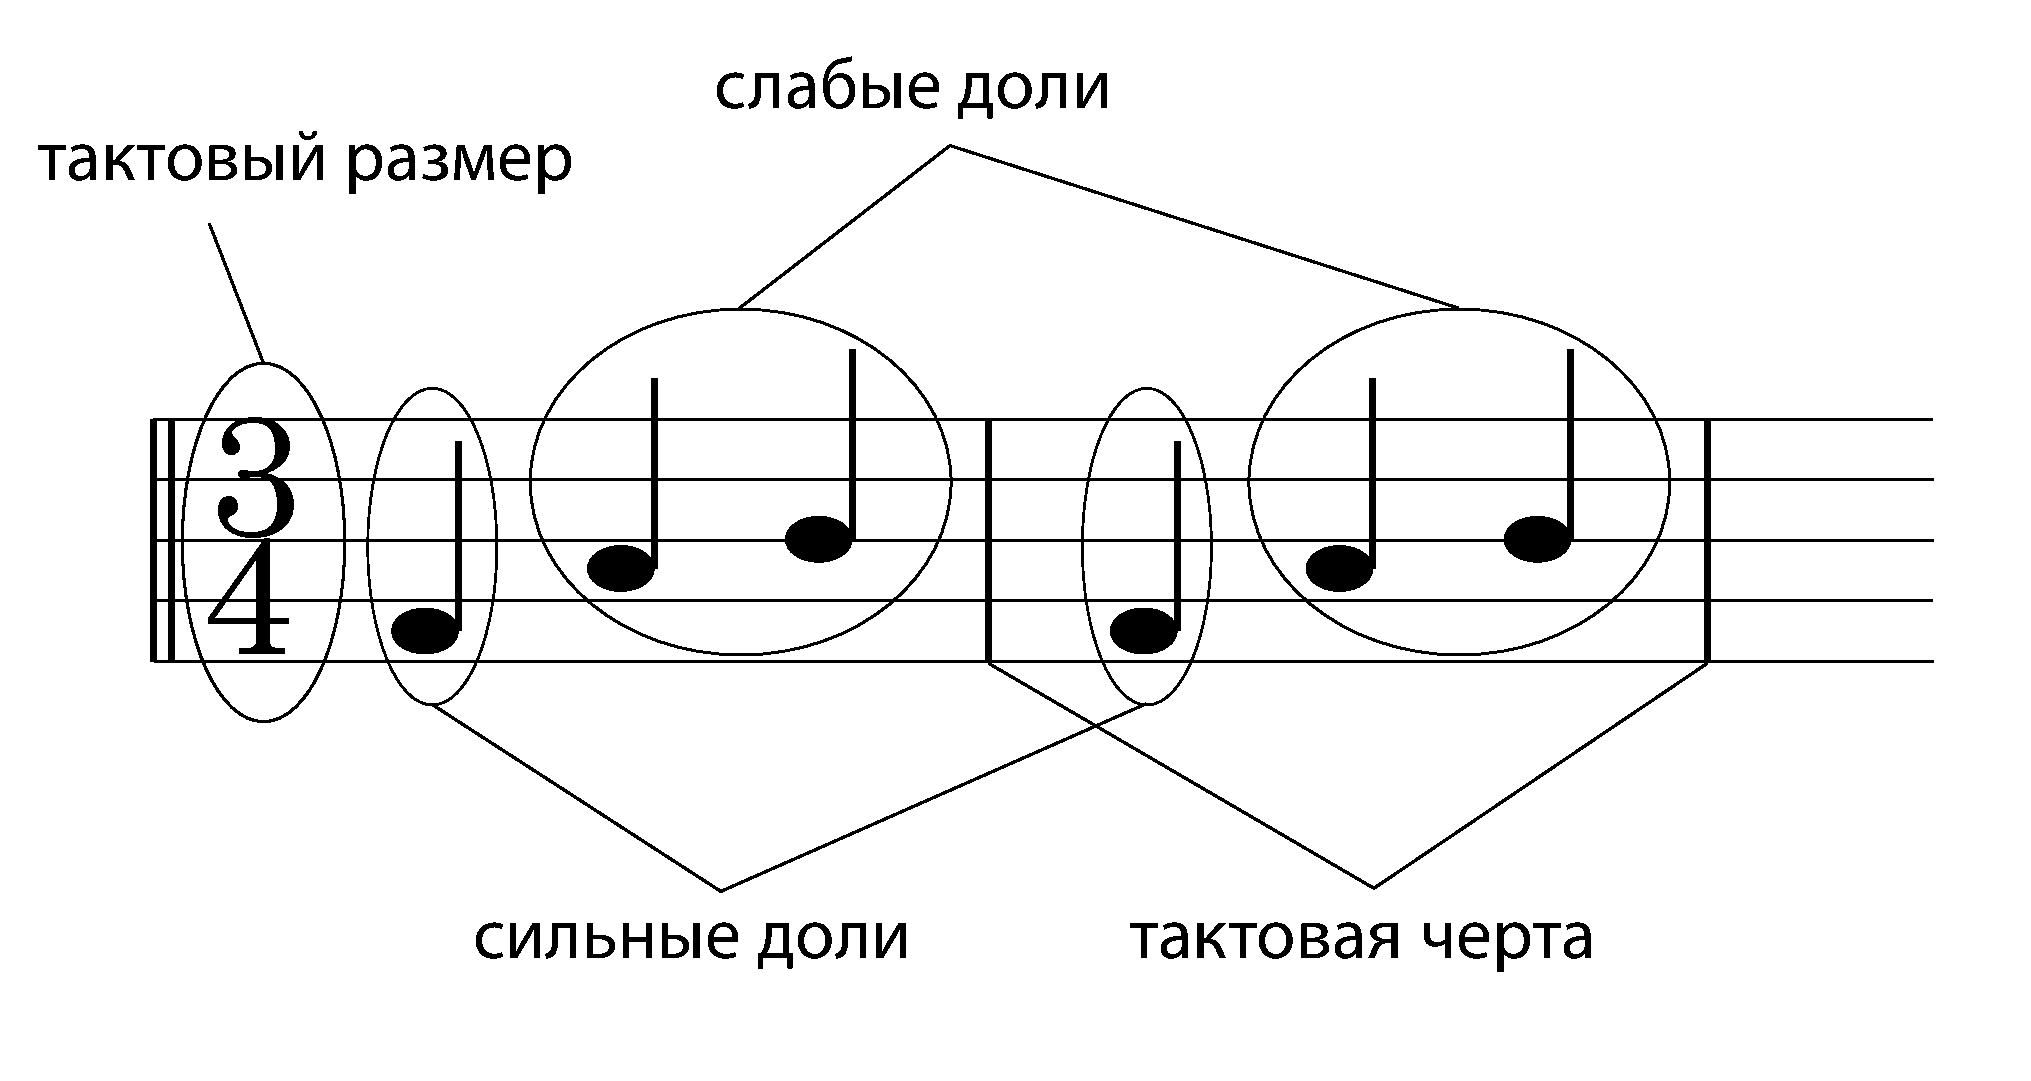
\includegraphics[scale=0.4]{svg/barlines.pdf}
	\end{center}
	\captionsetup{justification=centering}
	\caption{Обозначение метра}
	\label{img:meter}
\end{figure}

\newpage

Размер задает относительную длительность каждой доли. Например, размер <<3/4>> говорит о том, что в такте 3 доли, каждая из которых представлена четвертной нотой. Можно сказать, что размер -- числовое представление метра с указанием длительности каждой доли. Такт в свою очередь -- единица метра, начинающаяся с наиболее сильной доли и заканчивающаяся перед следующей равной ей по силе (рис.~\ref{img:meter}).

В данной работе не будут учитываться тонкости различия ритма и метра. Соответственно, для измерения ритма будет использоваться числовое представление метра в виде тактового размера.

\subsection{Проблема определения ритма и темпа}

Основной проблемой автоматического определения ритма и темпа музыки является наличие некоторых особенностей в музыкальных записях с живыми инструментами, затрудняющих это определение. Одна из таких особенностей -- это нечеткое попадание инструмента в ритмическую сетку. Такие небольшие отклонения на живых записях присутствуют всегда~\cite{quantize}. Они не заметны для уха человека, но могут осложнять автоматическое распознавание.

Также в некоторых случаях темп и ритм может изменяться в течение музыкального произведения. Пример переменного темпа приведен на рис.~\ref{img:aerials} (темп обозначается числами сверху в bpm). На рис.~\ref{img:master} приведен пример переменного ритма (размера).

\begin{figure}[h!]
	\begin{center}
		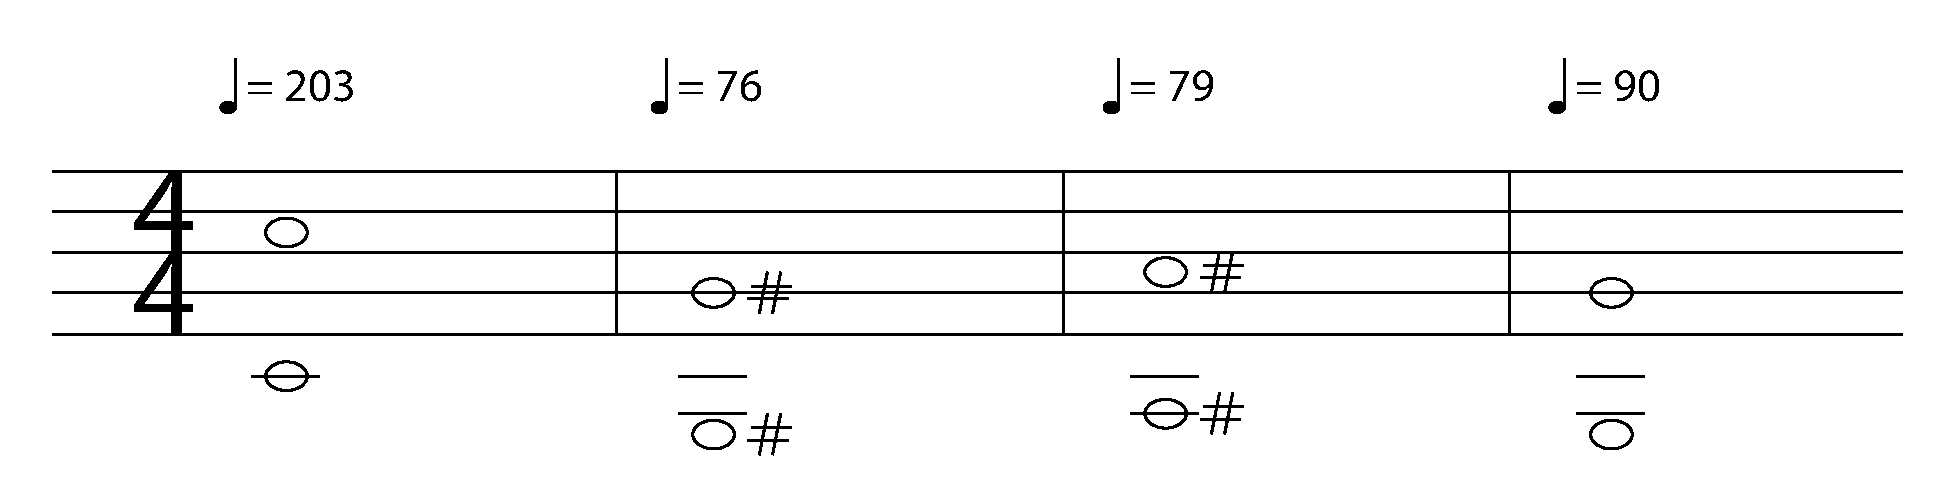
\includegraphics[scale=0.5]{svg/aerials.pdf}
	\end{center}
	\captionsetup{justification=centering}
	\caption{Пример переменного темпа (System of a down <<Aerials>>)}
	\label{img:aerials}
\end{figure}

\begin{figure}[h!]
	\begin{center}
		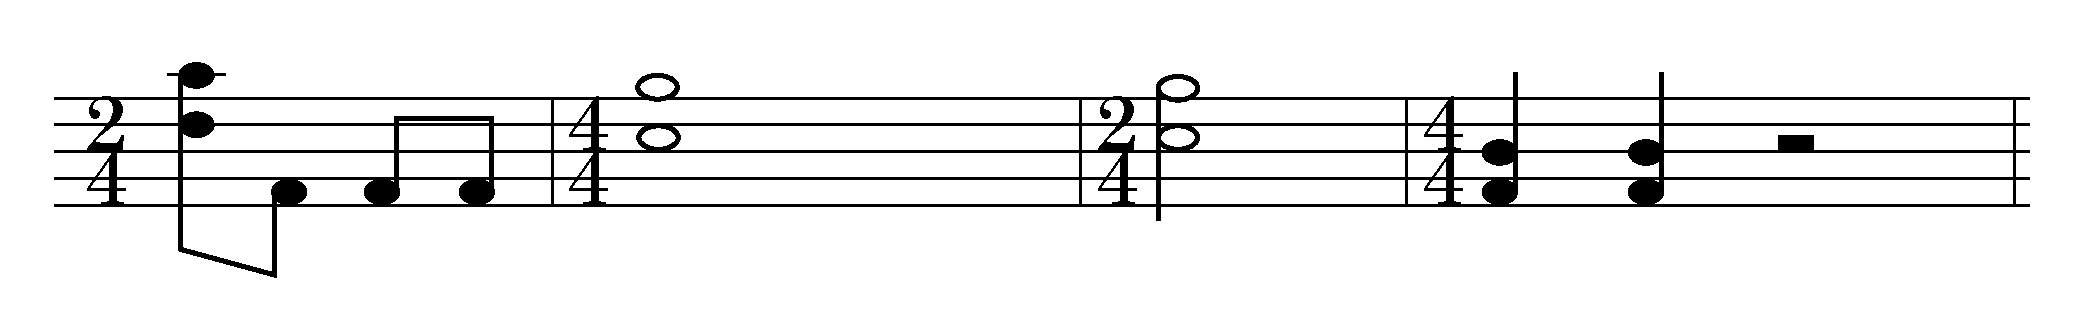
\includegraphics[scale=0.5]{svg/master.pdf}
	\end{center}
	\captionsetup{justification=centering}
	\caption{Пример переменного размера (Metallica <<Master of puppets>>)}
	\label{img:master}
\end{figure}

В качестве критериев сравнения рассматриваемых далее методов выделены следующие:

\begin{itemize}
	\item[--] точность результатов применения метода;
	\item[--] возможность определения переменного темпа и ритма;
	\item[--] ограничения на формат входного аудиофайла;
	\item[--] размер использовавшегося для обучения датасета (если обучение необходимо).
\end{itemize}

\subsection{Дискретное вейвлет-преобразование}

\subsubsection{Общие сведения}

Так как преобразование Фурье не позволяет получить частотно-временное представление сигнала, оно подходит только для стационарных сигналов (т. е. сигналов, частотное наполнение которых не меняется во времени). Большинство же реальных аудио-сигналов являются нестационарными. Основная же проблема оконного преобразования Фурье (ОПФ) заключается в невозможности получить произвольно точное частотно-временное представление сигнала, то есть нельзя определить для какого-то момента времени, какие спектральные компоненты присутствуют в сигнале. Эта проблема называется проблемой разрешения.

В качестве альтернативы ОПФ было разработано вейвлет-преобразование.

Основная идея вейвлет-преобразования -- это разделение сигнала на высокие и низкие частоты с помощью фильтров \cite{polikar}. После применения фильтров полученные низкие частоты снова пропускаются через два фильтра и т. д. При этом высокие частоты остаются неизменными. Эта операция называется декомпозицией.

На высоких частотах лучше разрешение по времени, а на низких -- по частоте.

Фильтры для высоких и низких частот определяются следующими уравнениями \cite{dwt}:

\begin{equation}\label{eq:highpass}
	y_{high}[k] = \sum_{n=-\infty}^{\infty} x[n] g[2k-n],
\end{equation}

\begin{equation}\label{eq:lowpass}
	y_{low}[k] = \sum_{n=-\infty}^{\infty} x[n] h[2k-n],
\end{equation}

где $x[n]$ -- пропускаемый через фильтр сигнал (последовательность), $h[n]$ и $g[n]$ -- импульсные характеристики (отклик на единичный импульс) низкочастотного и высокочастотного фильтров соответственно, $k$ и $n$ -- целые числа, соответствующие отсчетам (теорема отсчетов~\cite{samples}).

В целом, процедура пропускания сигнала через фильтр соответствует математической операции свертки сигнала $x[k]$ и импульсной характеристики фильтра $h[k]$, которая определяется как:

\begin{equation}\label{eq:conv}
	x[k]*h[k] = \sum_{n=-\infty}^{\infty} x[n] h[k-n].
\end{equation}

Выражение $2k-n$ в формулах \ref{eq:highpass} и \ref{eq:lowpass} позволяет обрезать сигнал, тем самым увеличив его масштаб в два раза (т.~к. половина частот удаляется в результате фильтрации)~\cite{polikar}.

Само ДВП описывается формулой:

\begin{equation}\label{eq:dwt}
	W(j, k) = \sum_{j}\sum_{k} x(k) 2^{-j/2} \psi(2^{-j}n-k),
\end{equation}

где $\psi(t)$ -- функция преобразования, называемая материнским вейвлетом, $j$ и $k$ связаны с параметрами сдвига $\tau$ (местоположение окна) и масштаба $s$ (величина, обратная частоте). $s = s_0^j$, $\tau = k s_0^j \tau_0$. В данном случае $s_0 = 2$, $\tau_0 = 1$.

\subsubsection{Определение ритма и темпа}

Алгоритм определения ритма с помощью ДВП основан на обнаружении наиболее заметных периодов сигнала.

Сигнал сначала раскладывается на несколько частотных полос с помощью ДВП. Для этого сигнал <<делится>> пополам на высокие и низкие частоты, после чего низкие частоты снова разделяются пополам и т.~д. Так продолжается до тех пор, пока не останутся два отсчета. Эта операция необходима, т.~к. для высоких частот можно точнее указать их временную позицию, а для низких -- их значение частоты~\cite{polikar}. После этого огибающая амплитуды во временной области каждой полосы извлекается отдельно. Это достигается за счет фильтрации нижних частот каждой полосы, применения полноволнового выпрямления и понижения частоты дискретизации \cite{dwt}. Затем огибающие каждой полосы суммируются и вычисляется автокорреляционная функция. Пики автокорреляционной функции соответствуют различным периодам огибающей сигнала.

Фильтрация нижних частот:

\begin{equation}
	y[n] = (1 - \alpha)x[n] - \alpha y[n],
\end{equation}

где $\alpha = 0,99$.

\newpage

Полноволновое выпрямление:

\begin{equation}
	y[n] = abs(x[n]).
\end{equation}

Понижение частоты дискретизации:

\begin{equation}
	y[n] = x[kn].
\end{equation}

Нормализация в каждой полосе (удаление среднего значения) для исключения аномальных данных:

\begin{equation}
	y[n] = x[n] - E[x[n]],
\end{equation}

где $E[x[n]]$ -- среднее значение последовательности $x[n]$.

Автокорреляция:

\begin{equation}
	y[k] = \frac{1}{N} \sum_{n=0}^{N-1}x[n]x[n+k].
\end{equation}

Из результата берутся первые пять пиков автокорреляционной функции, после чего рассчитываются и добавляются в гистограмму соответствующие им периодичности в bpm. Этот процесс повторяется в процессе прохождения по сигналу. Периодичность, соответствующая наиболее заметному пику конечной гистограммы, является предполагаемым темпом аудиофайла в bpm.

Основными недостатками рассмотренного метода определения темпа являются неточные (в некоторых случаях даже ошибочные) результаты на музыке определенных жанров (например, на классической музыке), а также невозможность определить переменный темп.

\subsection{Скрытые модели Маркова}

\subsubsection{Стохастическое моделирование}

Как уже было упомянуто выше, практически во всех музыкальных записях имеет место небольшое отклонение нот от ритмической сетки. Рассматриваемый метод рассчитан именно на работу с такими случаями. Также в данном методе подразумевается, что входные данные представлены в формате MIDI (Musical Instrument Digital Interface, стандарт обмена данными между цифровыми музыкальными инструментами). В MIDI файлах указывается информация о высоте ноты, ее длительности и силе нажатия~\cite{midi}.

Исследования показывают, что отклонения нот можно смоделировать с помощью распределения Гаусса относительно их идеальной длительности~\cite{hmm}. Тогда, если $i$ -- идеальная длительность ноты (<<намерение>>) в момент времени $t$, то ее исполненная длительность $x_t$ моделируется функцией плотности вероятности $f_i(x_t)$.

Пусть $Q = \{q_1, q_2, ..., q_N\}$ -- последовательность <<намерений>> в соответствующие моменты времени. Тогда наблюдаемая последовательность длительностей $X = \{x_1, x_2, ..., x_N\}$ определяется как:

\begin{equation}
	P(X|Q) = \prod_{t=1}^N f_{q_t}(x_t).
\end{equation}

В данном методе используются два типа моделей генерации ритмических рисунков для получения возможных ритмов:

\begin{itemize}
	\item[--] n-граммная модель (длина ноты предсказывается исходя из предыдущих n-1 нот в вероятностном смысле. Эта модель охватывает любые ритмические рисунки и может выдавать точную вероятность);
	\item[--] <<ритмический словарь>> (состоит из всех известных ритмических рисунков за единицу времени. Хорошо представляет известные ритмические рисунки, в то время как неизвестные заменяются аналогичными существующими ритмами).
\end{itemize}

Обе модели можно представить в виде вероятностных сетей перехода состояний, где каждое состояние связано с предполагаемой длительностью ноты. Вероятность того, что номер состояния изменится в последовательности $Q = \{q_1, q_2, ..., q_N\}$ определяется как $P(Q) = p_{q_0} \prod_{t=1}^N a_{q_{t-1}q_t}$, где $p_i$ -- вероятность изначального нахождения в состоянии $i$, а $a_{ij}$ -- вероятность перехода из состояния $i$ в состояние $j$.

Колеблющиеся длительности и возможные последовательности нот могут быть объединены в рамках скрытой модели Маркова как вероятности перехода $A = \{a_{ij}\}$ и наблюдаемые вероятности $B = \{b_i(x_t)\}$ соответственно. В таком случае вероятность наблюдения последовательности длительностей $X$ определяется как:

\begin{equation}
	P(X) = P(X|Q)P(Q).
\end{equation}

\subsubsection{Определение ритма}

Задача заключается в том, чтобы найти временную последовательность $Q$ номеров состояний, которая дает максимальную апостериорную вероятность $P(Q|X)$ при заданной последовательности наблюдаемых длительностей $X$~\cite{hmm}.

По теореме Байеса:

\begin{equation}
	P(Q|X) = \frac{P(X|Q)P(Q)}{P(X)}.
\end{equation}

Значит, максимизация апостериорной вероятности эквивалентна нахождению $argmax P(X|Q)P(Q)$ среди всех возможных $Q$.

Оптимальная последовательность состояний находится с помощью алгоритма Витерби для поиска наилучшего пути в вероятностной сети переходов.

Основной недостаток представленного метода заключается в необходимости входных данных быть в формате MIDI. Также к недостаткам можно отнести периодические неточности в результатах. Например, музыкальные фрагменты с разным темпом (к примеру, 116 bpm и 127 bpm) могут быть определены как имеющие одинаковый темп (в данном случае 120 bpm~\cite{hmm}).

\subsection{Байесовское иерархическое моделирование}

\subsubsection{Языковая модель}

Байесовское иерархическое моделирование состоит из двух компонентов: языковой модели (<<language>> model) и модели представления (<<performance>> model)~\cite{bayesian}.

Языковая модель построена на марковской модели нотных паттернов. В этой модели используется последовательность $B_k = z_{k,1}, ..., z_{k,l}$, где $k = 1, ..., K$ -- индекс в множестве нотных паттернов длины $K$, $z_{k,l}$ -- нота под номером $l$ в нотном паттерне $k$, где $l = 1, ..., L$, а $L$ -- количество нот в паттерне. При этом вероятность последовательности паттернов $w_{1:I} = w_1, ..., w_I$, где $w_i \in \{B_k\}_{k=1}^K$ определяется как:

\begin{equation}\label{eq:note_pattern}
	P(w_{1:I}) = P(w_1 = B_k) \prod_{i=2}^I P(w_i=B_{k'}|w_{i-1}=B_k).
\end{equation}

Проблемой этой модели в чистом виде является обработка синкоп (смещения акцента с сильной доли такта на слабую~\cite{syncope}), поскольку синкопированная нота лежит за границей такта, которая обычно является границей нотных паттернов.

\textbf{Модификация нотных паттернов}

Пусть $z_{1:M}$ -- последовательность нот, являющаяся результатом модели нотных паттернов, $y_{1:N}$ -- модифицированная последовательность $z_{1:M}$ (со вставленными нотами), а $x_{1:N}$ -- итоговая последовательность нот, получающаяся в результате языковой модели (содержащая в т.~ч. синкопы).

Синкопы могут быть интегрированы в модель путем расширения пространства состояний базовой модели $w_i$ до пары $(w_i; s_i)$, где $s_i$ -- степень синкопирования i-ой ноты (степень ее сдвига). Тогда выражение \ref{eq:note_pattern} изменяется как:

\begin{equation}
	P(w_{1:I}, s_{1:I}) = P(w_1 = B_k, s_1) \prod_{i=2}^I P(w_i=B_{k'}, s_i|w_{i-1}=B_k, s_{i-1}).
\end{equation}

\textbf{Процесс Дирихле}

Поскольку используемые нотные паттерны и типы модификаций варьируются в зависимости от музыкальных произведений, для отдельных произведений учитываются разные значения параметров. В байесовской модели эти параметры считаются сгенерированными из предшествующих (априорных) моделей. Процесс Дирихле~\cite{dirichlet} может служить этой априорной моделью.

Пусть $\pi_{kk'} = P(w_i=B_{k'}|w_{i-1}=B_k)$. В случае конечных распределений процесс Дирихле для дискретного распределения $\pi$ описывается базовым распределением $\omega$ и параметром концентрации $\alpha$ следующим образом:

\begin{equation}
	\pi \sim Dir(\alpha\omega),
\end{equation}

где $Dir()$ обозначает распределение Дирихле.

Когда параметр концентрации $\alpha$ мал, используется компактная грамматика, т.~е. для каждого музыкального произведения будет использоваться небольшое количество паттернов нот.

\subsubsection{Модель представления}

Модель описывает два источника <<колебаний>> (неточностей) в музыкальном исполнении. Один из них -- колебание ритма, а другой -- колебание темпа~\cite{bayesian}. Пусть $v_i = d_i / x_i$, где $x_i$ -- <<формальная>> длительность i-ой ноты, а $d_i$ -- фактический интервал между i-ой и (i+1)-ой нотами. Вариация $v_i$ описывается марковским процессом. Предполагая, что колебания темпа и ритма являются гауссовскими, модель представления задается как:

\begin{equation}
	\begin{cases}
		v_n|v_{n-1} \sim N(v_{n-1}, \sigma_v^2),\\
		d_n|v_n, x_n \sim N(v_nx_n, \sigma_t^2),
	\end{cases}
\end{equation}

где $\sigma_v$ ($\sigma_t$) -- стандартное отклонение для колебаний темпа (ритма).

Полная вероятность для модели представления задается как:

\begin{equation}
	P(d_{1:N}, v_{1:N}|x_{1:N}) = \prod_{n=1}^N P(d_n|v_n, x_n)P(v_n|v_{n-1}),
\end{equation}

где $P(v_1|v_0) \equiv P(v_1)$.

Таким образом, байесовское иерархическое моделирование позволяет немного увеличить точность определения ритма по сравнению с марковскими моделями (примерно на 2\%~\cite{bayesian}). Но остальные недостатки скрытых марковских моделей остаются прежними: работа только с MIDI форматами и определение только постоянного темпа.

\subsection{Использование сверточных нейросетей}

\subsubsection{Представление сигнала}

Сигнал представляется в виде спектрограммы по шкале мела, чтобы снизить объем данных, который должен быть обработан нейросетью (мел, от слова <<мелодия>>, - психофизическая (субъективная) единица высоты звука~\cite{mels}). Шкала мела выбрана вместо линейной шкалы из-за ее связи с человеческим восприятием и диапазонами частот инструментов.

Чтобы создать спектрограмму, сигнал конвертируется в моно, его дискретизация понижается до 11025~Гц, после чего используются полуперекрывающиеся окна из 1024 отсчетов~\cite{cnn}. Это эквивалентно частоте кадров 21,5~Гц, что (согласно теореме отсчетов) достаточно для представления темпа до 646 bpm. Каждое окно преобразуется в 40-полосный спектр в шкале мел, охватывающий диапазон от 20 до 5000~Гц. В качестве длины спектрограммы выбрано 256 кадров, что примерно равняется 11,9~с.

\subsubsection{Архитектура сети}

Архитектура рассматриваемой сети представлена на рис.~\ref{img:cnn}.

Сначала входные данные обрабатываются тремя сверточными слоями, каждый из которых состоит из 16 фильтров размера 1х5. С помощью этих фильтров сопоставляется ритмическая структура сигнала.

После этого идут четыре модуля с несколькими фильтрами. Каждый из модулей состоит из среднего слоя пулинга (<<avg pooling>>), шести параллельных сверточных слоев с фильтрами разных размеров (от 1х32 до 1х256), слоя конкатенации и т.~н. <<узкого>> (<<bottle-neck>>) слоя, предназначенного для уменьшения размерности. С помощью этих модулей достигаются две цели:

\begin{enumerate} 
	\item Пулинг по оси частот для суммирования диапазонов мел.
	\item Сопоставление сигнала с различными фильтрами, способными обнаруживать длительные временные зависимости.
\end{enumerate}

Чтобы классифицировать свойства, полученные из сверточных слоев, добавляются два полносвязных слоя (по 64 единицы каждый), за которыми следует выходной слой с 256 единицами. Выходной слой использует softmax в качестве функции активации, а все остальные слои используют ELU~\cite{elu}. Каждому сверточному или полносвязному слою предшествует пакетная нормализация~\cite{batch}. Первому полносвязному слою также предшествует слой отсева с $p = 0,5$ (<<dropout>>) для противодействия переобучению.

\begin{figure}[h!]
	\begin{center}
		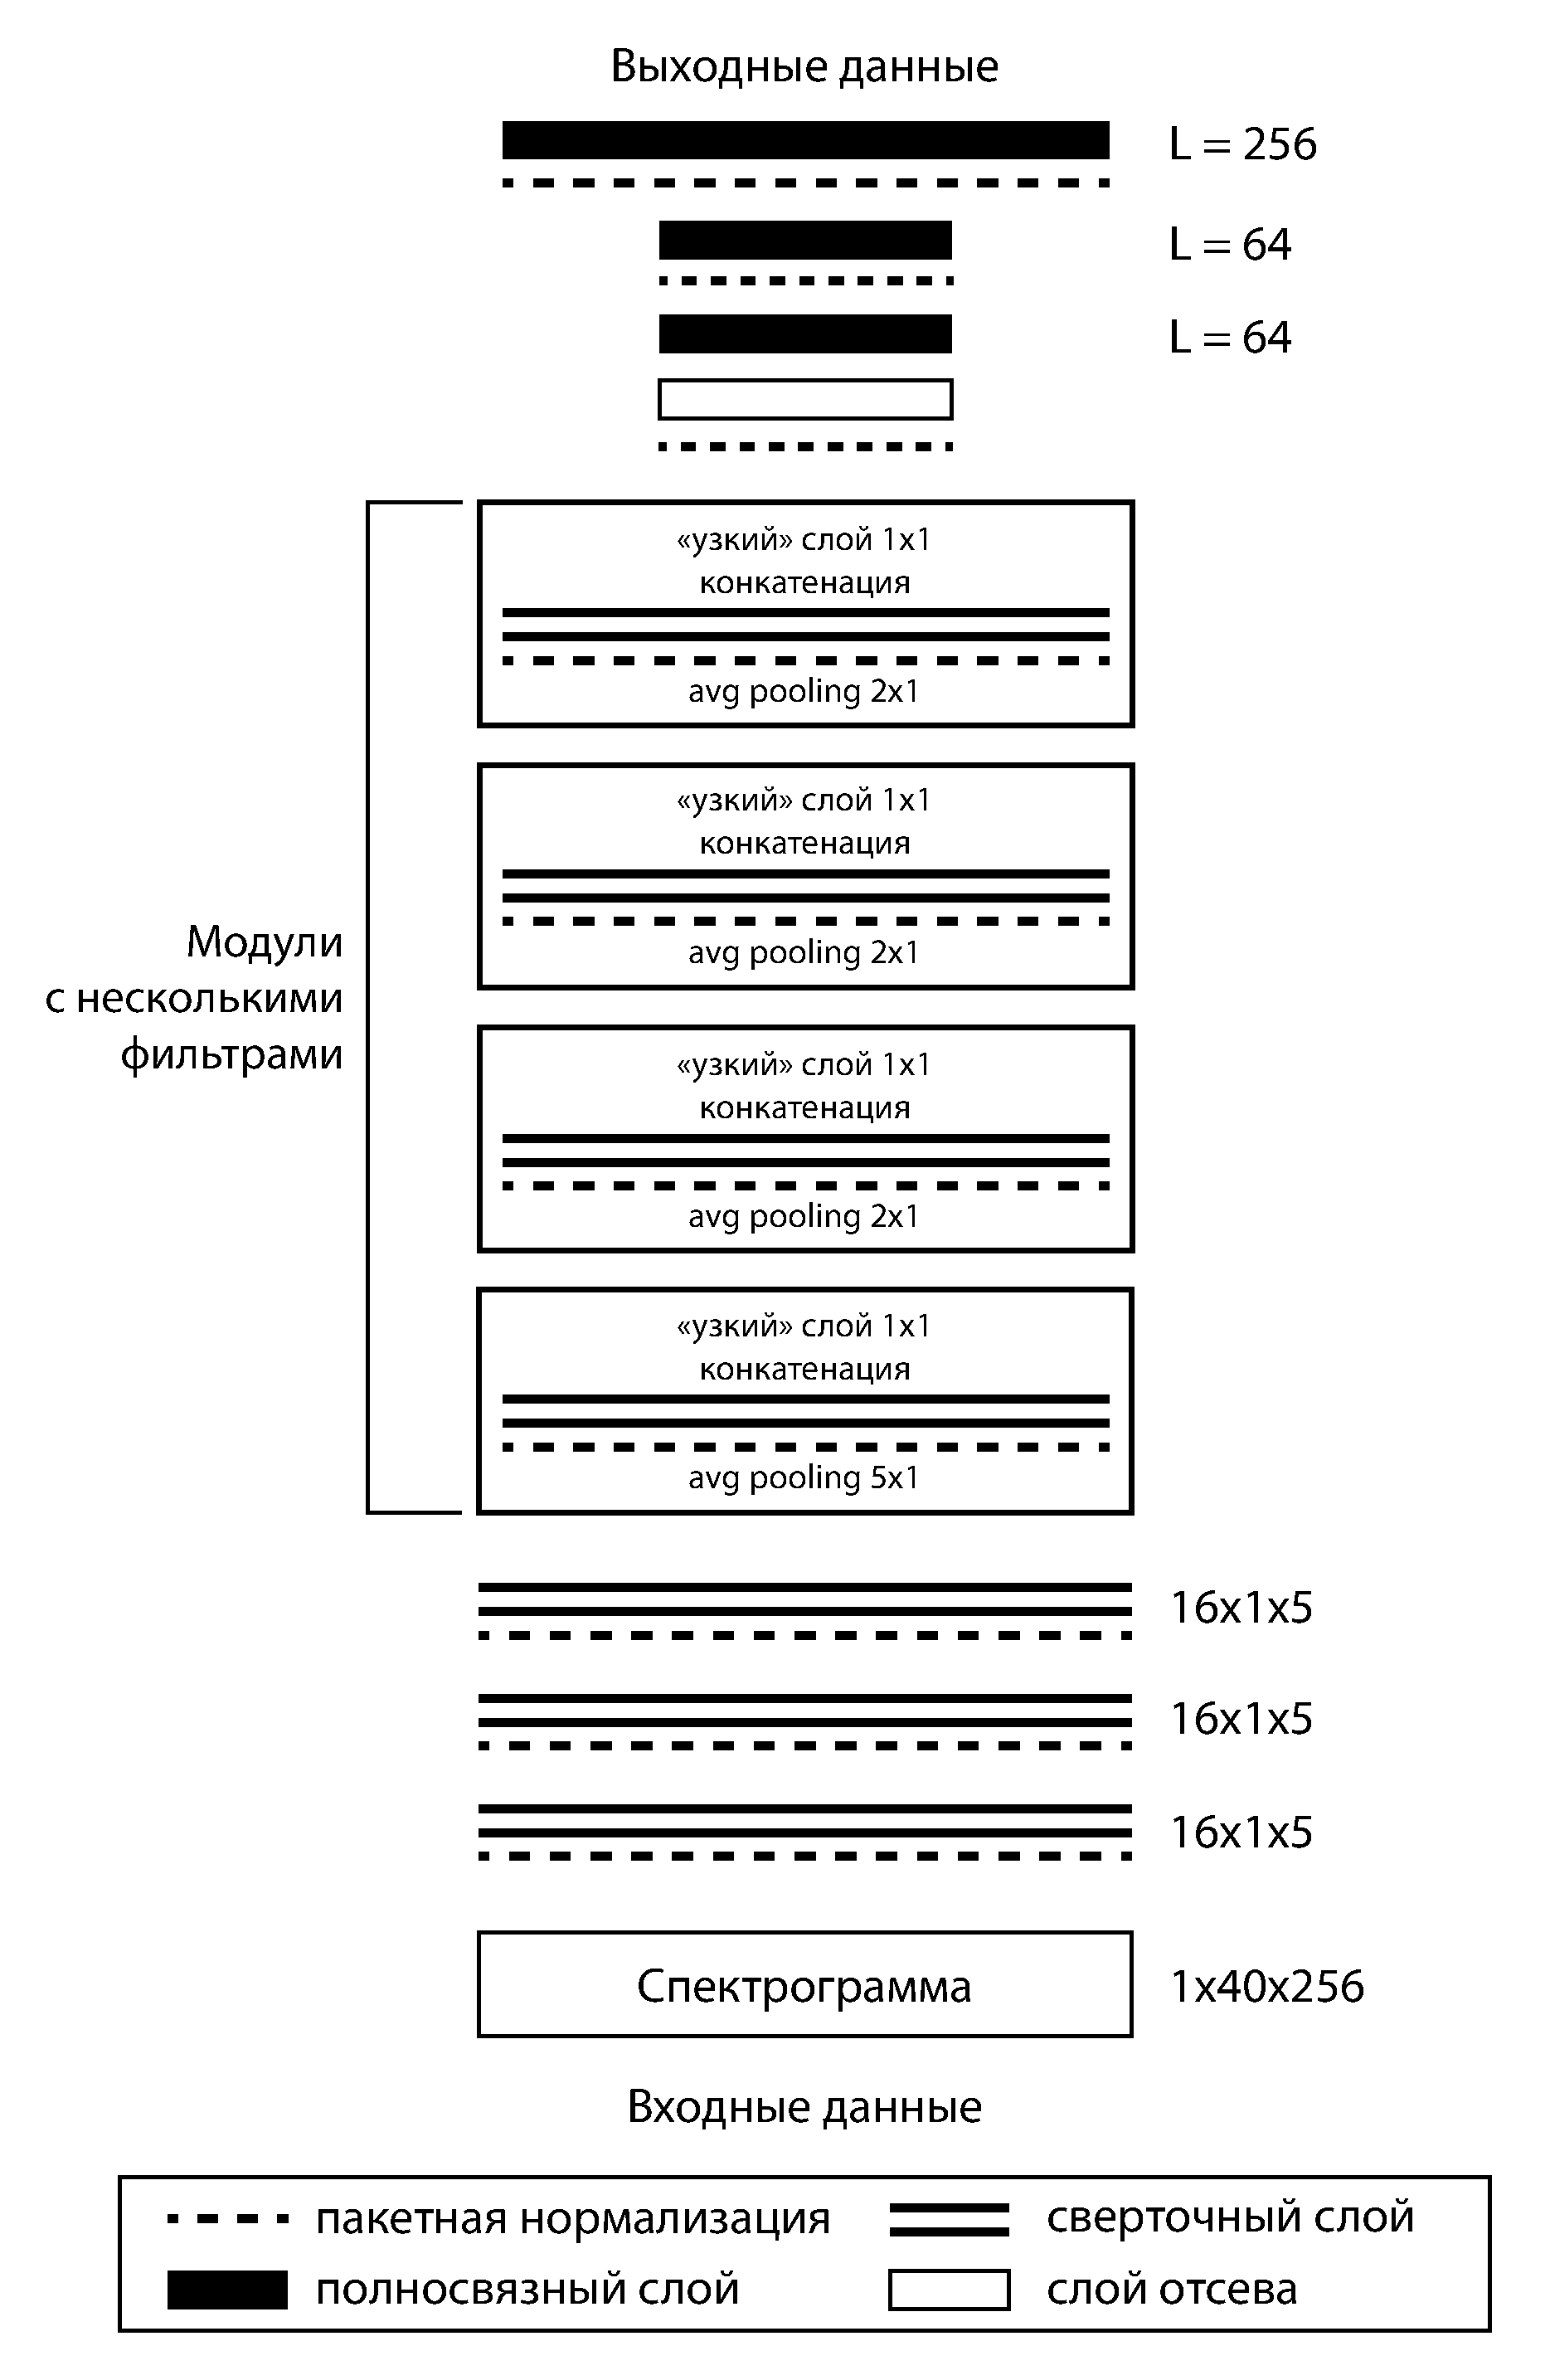
\includegraphics[scale=0.33]{svg/cnn.pdf}
	\end{center}
	\captionsetup{justification=centering}
	\caption{Схема архитектуры нейросети}
	\label{img:cnn}
\end{figure}

\newpage

Всего сеть имеет 2921042 обучаемых параметра.

В результате выбирается один из 256 вариантов темпа от 30 до 285 bpm.

Таким образом, сверточные нейросети позволяют определять темп с достаточно высокой точностью (до 98\%~\cite{cnn}). Также данный метод можно использовать и при определении глобального темпа, не только для фрагментов. Но он по-прежнему не позволяет определить переменный темп, а также не предназначен для определения ритма. Помимо этого нейросетевые методы имеют такие недостатки, как необходимость обучающих датасетов больших объемов, зависимость от исходных данных и долгое время обучения.

\subsection{Сравнение методов}

По результатам рассмотрения перечисленных выше методов была составлена таблица \ref{tbl:compare}.

Как видно из таблицы, ни один метод в своем изначальном варианте не предполагает определение переменного темпа и ритма. Однако метод скрытых марковских моделей при небольшой модификации может позволить определить переменный темп и ритм~\cite{hmm}.

Также стоит заметить, что все методы, кроме ДВП, содержат обучаемые параметры. В скрытых марковских моделях -- это множество $\{a_{ij}\}$, а в байесовском иерархическом моделировании -- множество $\{\pi_{kk'}\}$. В обоих методах обучение происходит с помощью статистической оценки. Размеры датасетов в таблице были указаны исходя из данных, использовавшихся для обучения соответствующих моделей в исследованиях.

\begin{table}[h!]
	\begin{center}
		\caption{\label{tbl:compare}Сравнение рассмотренных методов}
		\begin{tabular}{|p{2.5cm}|p{2.5cm}|p{3cm}|p{3cm}|p{3cm}|}
			\hline
			Метод & Точность результатов & Переменный темп и ритм & Формат входного аудиофайла & Размер использовавшегося датасета \\\hline
			ДВП & Сильно зависит от жанра & Не определяются  & Нет ограничений & Обучение не требуется\\\hline
			Скрытые марковские модели & Разный темп может определяться как одинаковый  & Могут определяться при модификации метода & MIDI & 88~\cite{hmm}\\\hline
			Байес & Выше марковских примерно на 2\% & Не определяются  & MIDI & 100~\cite{bayesian}\\\hline
			Сверточная нейросеть & до 98\%  & Не определяются  & Нет ограничений & 3611~\cite{cnn}\\\hline
		\end{tabular}
	\end{center}
\end{table}

\newpage

\subsection*{Выводы}

В этом разделе была проанализирована предметная область и сформулирована проблема. А также была проведена классификация и сравнение основных существующих методов решения поставленной задачи.


